\chapter{Разработка и исследование преобразователя силы на основе Velostat}\label{ch:ch3}

Третья глава содержит описание этапов разработки и исследования пьезорезистивного тактильного преобразователя силы на основе материала Velostat. Тактильное очувствление является основным способом получения информации о геометрии и физических свойствах опорной поверхности по которой движется робот в условиях отсутствия видимости. Именно для шагающих аппаратов, в отличие от колёсных и гусеничных, такой способ является актуальным, поскольку ноги робота используются одновременно и как движители, и как устройства для ощупывания поверхности. В главе обосновано применения преобразователя силы на основе полимерного материала Velostat, представлены экспериментальные исследования работы преобразователя при площади нагрузки меньше
размеров самого преобразователя, что имитирует условия контакта ног шагающего робота с жесткой опорной
поверхностью, по результатам экспериментальных исследований показано при каких условиях характеристики преобразователя удовлетворяют требованиям к системе тактильного восприятия шагающего робота.

Среди возможных способов определения силы реакции опоры наиболее целесообразным представляется её измерение с помощью датчиков силы, расположенных непосредственно в зоне контакта ноги с опорной поверхностью. Среди доступных датчиков такого типа большинство обладают излишней чувствительностью и точностью, а также имеют очень высокую стоимость, что делает их применение неоправданным для использования в роботах, предназначенных для изучения труднодоступных мест, в которых высока вероятность потери робота. В связи с этим, предложено использовать преобразователь силы на базе материала Velostat. Первоначально Velostat был разработан как упаковочный материал, изготовленный из полимерной пленки (полиолефины), пропитанной сажей для придания ей электропроводности. Свойство изменять свое сопротивление при изгибе или давлении сделало материал популярным решением для изготовления недорогих
датчиков давления [120]. Такой датчик позволяет решить проблемы классификации местности и создания карт на биомиметическом многоногом роботе StriRus. Velostat обладает вязкоупругим поведением, а также свойствами квантового туннелирования и предварительной локализации, что существенно влияет на отклик датчика. Но при исследовании разработанного преобразователя, была замечена зависимость в результатах показания преобразователя при разных площадях касаемой поверхности и рабочей области сенсора. Эту зависимость необходимо формализовать.

Система из нескольких датчиков усилия, расположенных на опорной поверхности ноги робота позволяет определить величину и точку приложения силы реакции опоры. В совокупности с показаниями датчиков тока, определяющих нагрузку на двигателях, датчиков поворота ног, определяющих конфигурацию шагающего робота, а также инерциальных датчиков, определяющих ускорения корпуса робота и, соответственно, изменение его скорости, положения и ориентации, это потенциально даёт необходимую информацию как для определения геометрической формы, так и некоторых физических свойств поверхности, по которой движется робот.

В мобильных роботах широко используются сенсорные системы, которые включают в себя инерциальные измерительные приборы (IMU), датчики тока двигателей, датчики силы, звуковые датчики, системы технического зрения и другие оптические сенсоры \cite{libby_using_2012,ojeda_terrain_2006,peters_analysis_2006}. Однако, для решения указанных задач в условиях плохой видимости, оптические системы становятся неработоспособны, и на первый план выходит использование датчиков силы. В обнаружении формы поверхности. Существует класс роботов (RHEX, Strirus), которые обладают такими параметрами.

Как было отмечено в предыдущих разделах, наиболее перспективным является применение разрабатываемого шагающего робота в пещерах, поверхность которой имеет неровности и  состоит из твердых и скользких поверхностей, ходовых грунтов. Для работы в таких местах робот должен получать информацию о физических свойствах местности. Эта информация оказывает существенное влияние на эффективность и стратегии локомоции. Например, на зернистой или травянистой местности взаимодействие между ногами и землей может привести к резкому рассеиванию энергии из-за трения. Это происходит из-за деформации поверхности ногами. Знание этой информации о взаимодействии ноги с землей может быть использовано для управления адаптацией.

Имея подробную информацию о взаимодействии ноги-земля, возможно решить множество задач, таких как идентификация местности \cite{wuIntegratedGroundReaction2016, walasTerrainClassificationLocomotion2016, mrva_feature_2015, dallaire_learning_2015}, управление походкой на основе рельефа местности \cite{wuTactileSensingTerrainBased2020, weingarten_automated_2004}, анализ устойчивости и SLAM \cite{odenthal_nonlinear_1999, peters_analysis_2006, Altendorfer2001}. Решение этих задач позволяет значительно повысить проходимость и возможности исследования мобильных роботов.


Существует несколько типов датчиков, которые могут измерять контактные силы и распределение давления. Это могут быть оптические, пьезорезистивные, пьезоэлектрические, магнитные, емкостные, на основе оптических волокон \cite{howe_dynamic_1993}. Промышленные датчики момента силы (F/T) широко распространены на гуманоидах (Atlas, Fedor) или четвероногих (Spot, AnyMal). Однако они слишком велики для небольших роботов, таких как RHEX, WHEGS или StriRus \cite{saranli_design_2000,schroerComparingCockroachWhegs2004, bulichevConceptDevelopmentBiomimetic2018}. Та же проблема применима к оптическим и магнитным датчикам. Емкостные датчики требуют высокой точности изготовления. В свою очередь, пьезорезистивные датчики имеют маленькие размеры, могут быть размещены практически на любой поверхности, имеют низкую стоимость и не требовательны к условиям эксплуатации.

Самый популярный тип пьезорезистивного датчика - тензодатчик. Он может быть установлен на ногах робота, но это решение требует наличия цепей формирования сигнала и создает трудности при прокладке проводов между постоянно вращающимися ногами и корпусом робота \cite{wuTactileSensingTerrainBased2020}. Другой способ - использовать пьезорезистивные датчики на основе проводящих волокон или полимеров. Они недорогие, очень гибкие и компактные. К сожалению, одной из распространенных проблем является значительный гистерезис. Было решено использовать Velostat (Linqstat)\cite{vehecFlexibleResistiveSensor2020} в качестве промежуточного слоя для резистивного датчика.

Velostat --- это вязкоупругое проводящее волокно. Вязкие материалы, такие как медь, при сопротивлении сдвигаются и натягиваются линейно во время напряжения. Упругие материалы тянутся во время растягивания и быстро возвращаются в обратное состояние, когда уходит напряжение. проявляются свойства обоих типов, что, по сути, приводит к постепенному  изменению напряжения в материале в зависимости от времени. Это резко влияет на отклик датчика.
Вязкоупругое поведение материала является высоко нелинейным, что влияет на получаемые данные с сенсора.

На основе данного материала был разработан и изготовлен пьезорезистивный датчик, где материал Velostat \pic{fig:velostat_sensor.jpg} является промежуточным слоем для датчика \pic{fig:simplest_sensor.jpg}. 

Для использования такого датчика необходимо оценить его поведение. Например, выяснено, что если приложить одинаковую точечную силу в разных точках датчика, результат измерений будет значительно отличаться. Чтобы понять, как с этим работать, нужно сформулировать и смоделировать сценарии использования.

\begin{figure}[H]
    \begin{subfigure}[t]{0.9\textwidth}
        \centering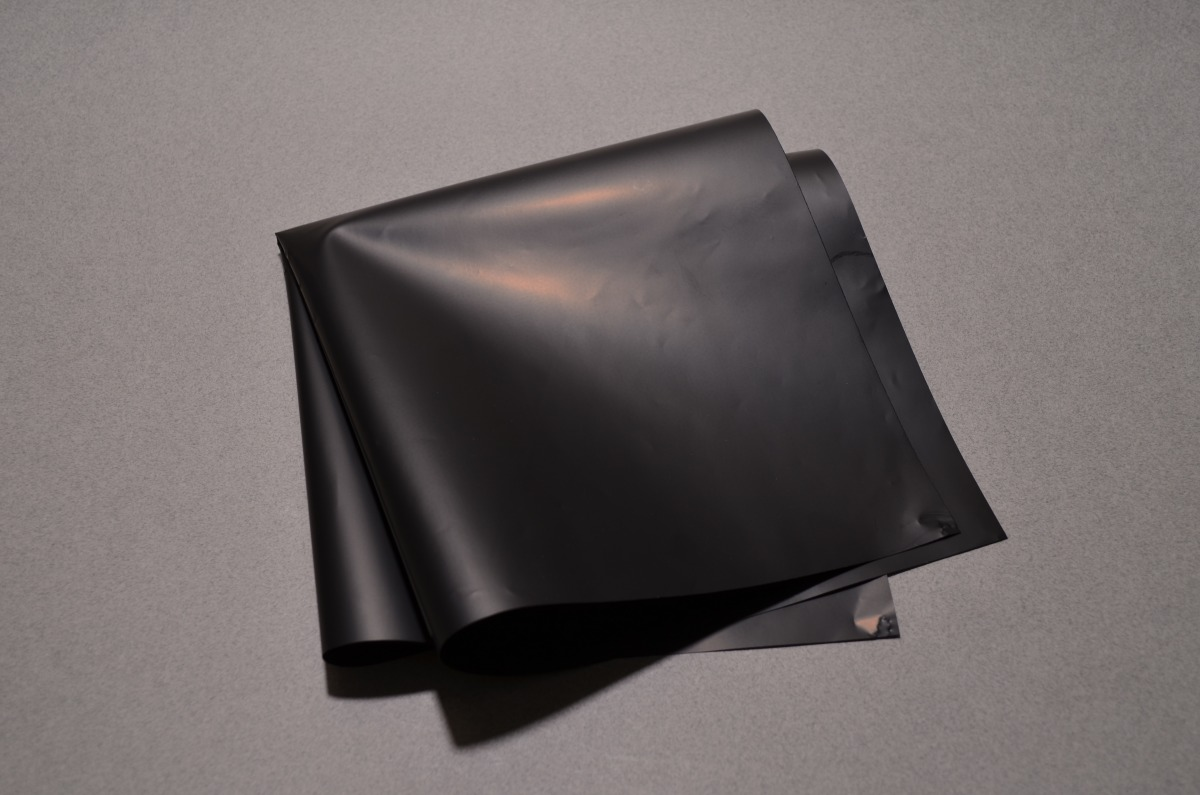
\includegraphics[height=8cm,width=1\textwidth,keepaspectratio]{velostat_sensor.jpg}
        \caption{Материал Velostat}
        \label{fig:velostat_sensor.jpg}
    \end{subfigure}

    \begin{subfigure}[t]{0.95\textwidth}
        \centering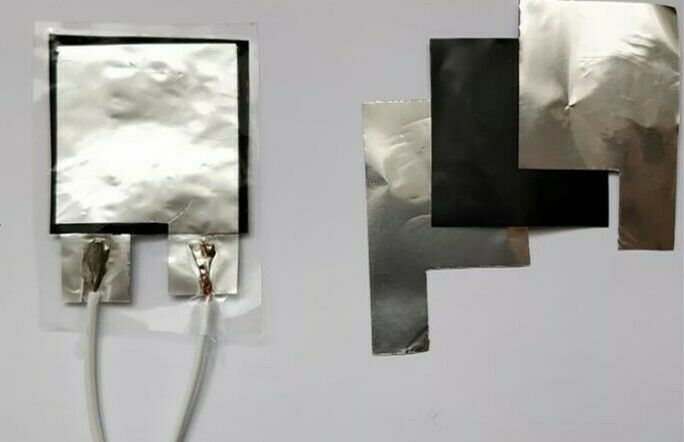
\includegraphics[height=8cm,width=1\textwidth,keepaspectratio]{simplest_sensor.jpg}
        \caption{Простейший преобразователь силы на основе Velostat}
        \label{fig:simplest_sensor.jpg}
    \end{subfigure}
    \caption{Примеры использования Velostat}
\end{figure}

При исследовании преобразователя силы на основе Velostat, было замечено, что площадь нажатия влияет на показания преобразователя. Поэтому актуальна задача изучения характеристик преобразователя , когда площадь касания меньше, чем размер сенсора.

\section{Физическая реализация преобразователя силы на основе Velostat}

Датчик состоит из двух медных оболочек, разделенных слоем Velostat. Давление на датчик приводит к изменению его сопротивления: чем выше давление, тем ниже сопротивление. Измеренное сопротивление Velostat образует делитель напряжения с постоянным резистором R1...R8 \pic{fig:el_scheme}.


\begin{figure}[H]
\centering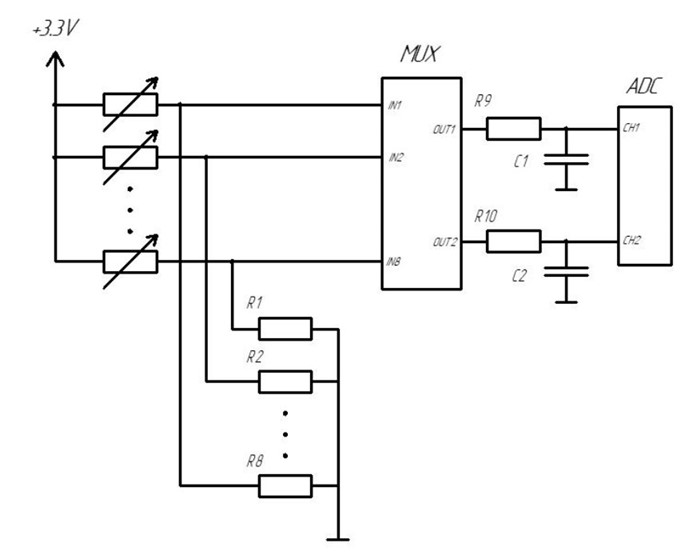
\includegraphics[width=0.8\textwidth]{electric_scheme.jpg}\\
\caption{Электрическая схема преобразователя силы}
\label{fig:el_scheme}
\end{figure}

На одну из пластин датчика подается напряжение 3,3 вольта. Таким образом, когда давление на датчик отсутствует (в идеальном случае сопротивление стремится к бесконечности), напряжение на выходе делителя стремится к нулю. По мере увеличения давления сопротивление будет уменьшаться, и напряжение на делителе будет приближаться к напряжению питания.

 Давление на датчик приводит к изменению его сопротивления: чем выше давление, тем ниже сопротивление. На \pic{fig:velostat_pressure_resistance.jpg} показана рабочая область сенсора, основанная на весе, который может быть приложен на одну ногу робота. Как видно из графика, сопротивление в рабочем диапазоне (5...6 кг) уменьшается незначительно. Для проведения измерений сопротивления с достаточной точностью номинал резисторов R1...R8 подбирается таким образом, чтобы обеспечить наклон зависимости напряжения на выходе делителя от сопротивления датчика в интересующем диапазоне.
\begin{figure}[H]
    \centering
    \begin{tikzpicture}
        % Include the image in a node
        \node [above right, inner sep=0] (image) at (0,0)
        {\centering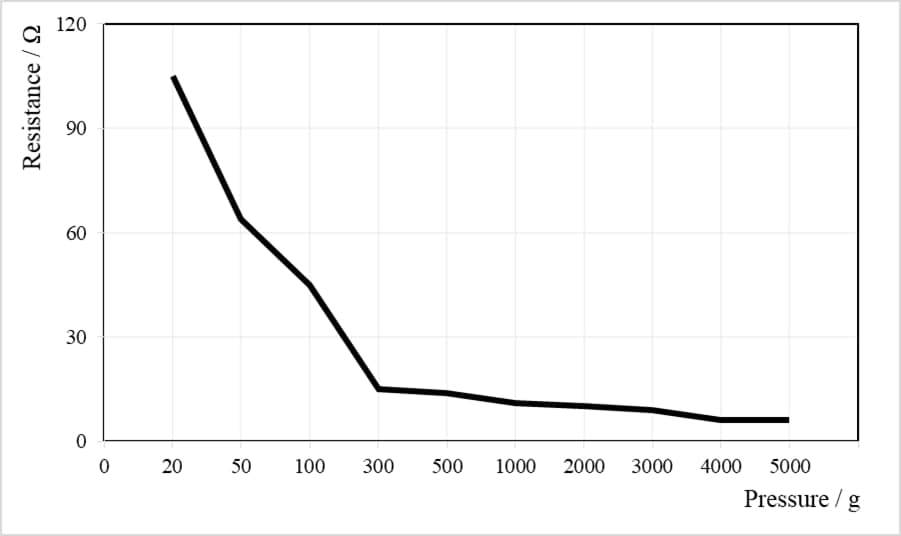
\includegraphics[height=10cm,width=1\textwidth,keepaspectratio]{velostat_pressure_resistance.jpg}};
        % Create scope with normalized axes
        \begin{scope}[
                x={($ 0.1*(image.south east)$)},
                y={($ 0.1*(image.north west)$)}]
            \draw[stealth-, very thick,green] (4.21,2.75) -- (6.5,5);
            \draw[stealth-, very thick,green] (8.75,2.15) -- (6.5,5)
            node[rounded corners=3pt,above,black,fill=white]{\small Рабочая область};
        \end{scope}
    \end{tikzpicture}
    \caption{График зависимости прикладываемого веса от сопротивления}
    \label{fig:velostat_pressure_resistance.jpg}
\end{figure}

\section{Разработка экспериментального стенда}

Исследования преобразователя Velostat, для случаев которых площадь нагрузки меньше, чем размер преобразователя, были проведены с помощью разработанного для этой цели исследовательского стенда. Основные требования к стенду включали в себя: необходимость контролировать силу нажатия и повторяемость эксперимента как по величине, так и по расположению площадки контакта инструмента и исследуемого преобразователя силы. Указанным требованиям возможно удовлетворить, используя коллаборативный робот-манипулятор, который будет управляться с помощью импедансного управления.

Использование коллаборативного робота позволяет также удовлетворить требованиям безопасности и допустить работу робота в непосредственно близости от экспериментатора. Разработанный стенд, представлен на рисунке \ref{fig:exp_standd}. Ссылка на видео работы стенда \quad \qrcode[height=1.5cm]{https://youtu.be/Gw4wVZ-ESuE}

\begin{figure}[H]
    \centering
        \begin{subfigure}{0.9\textwidth}
            \begin{tikzpicture}
                % Include the image in a node
                \node [
                    above right,
                    inner sep=0] (image) at (0,0) {\centering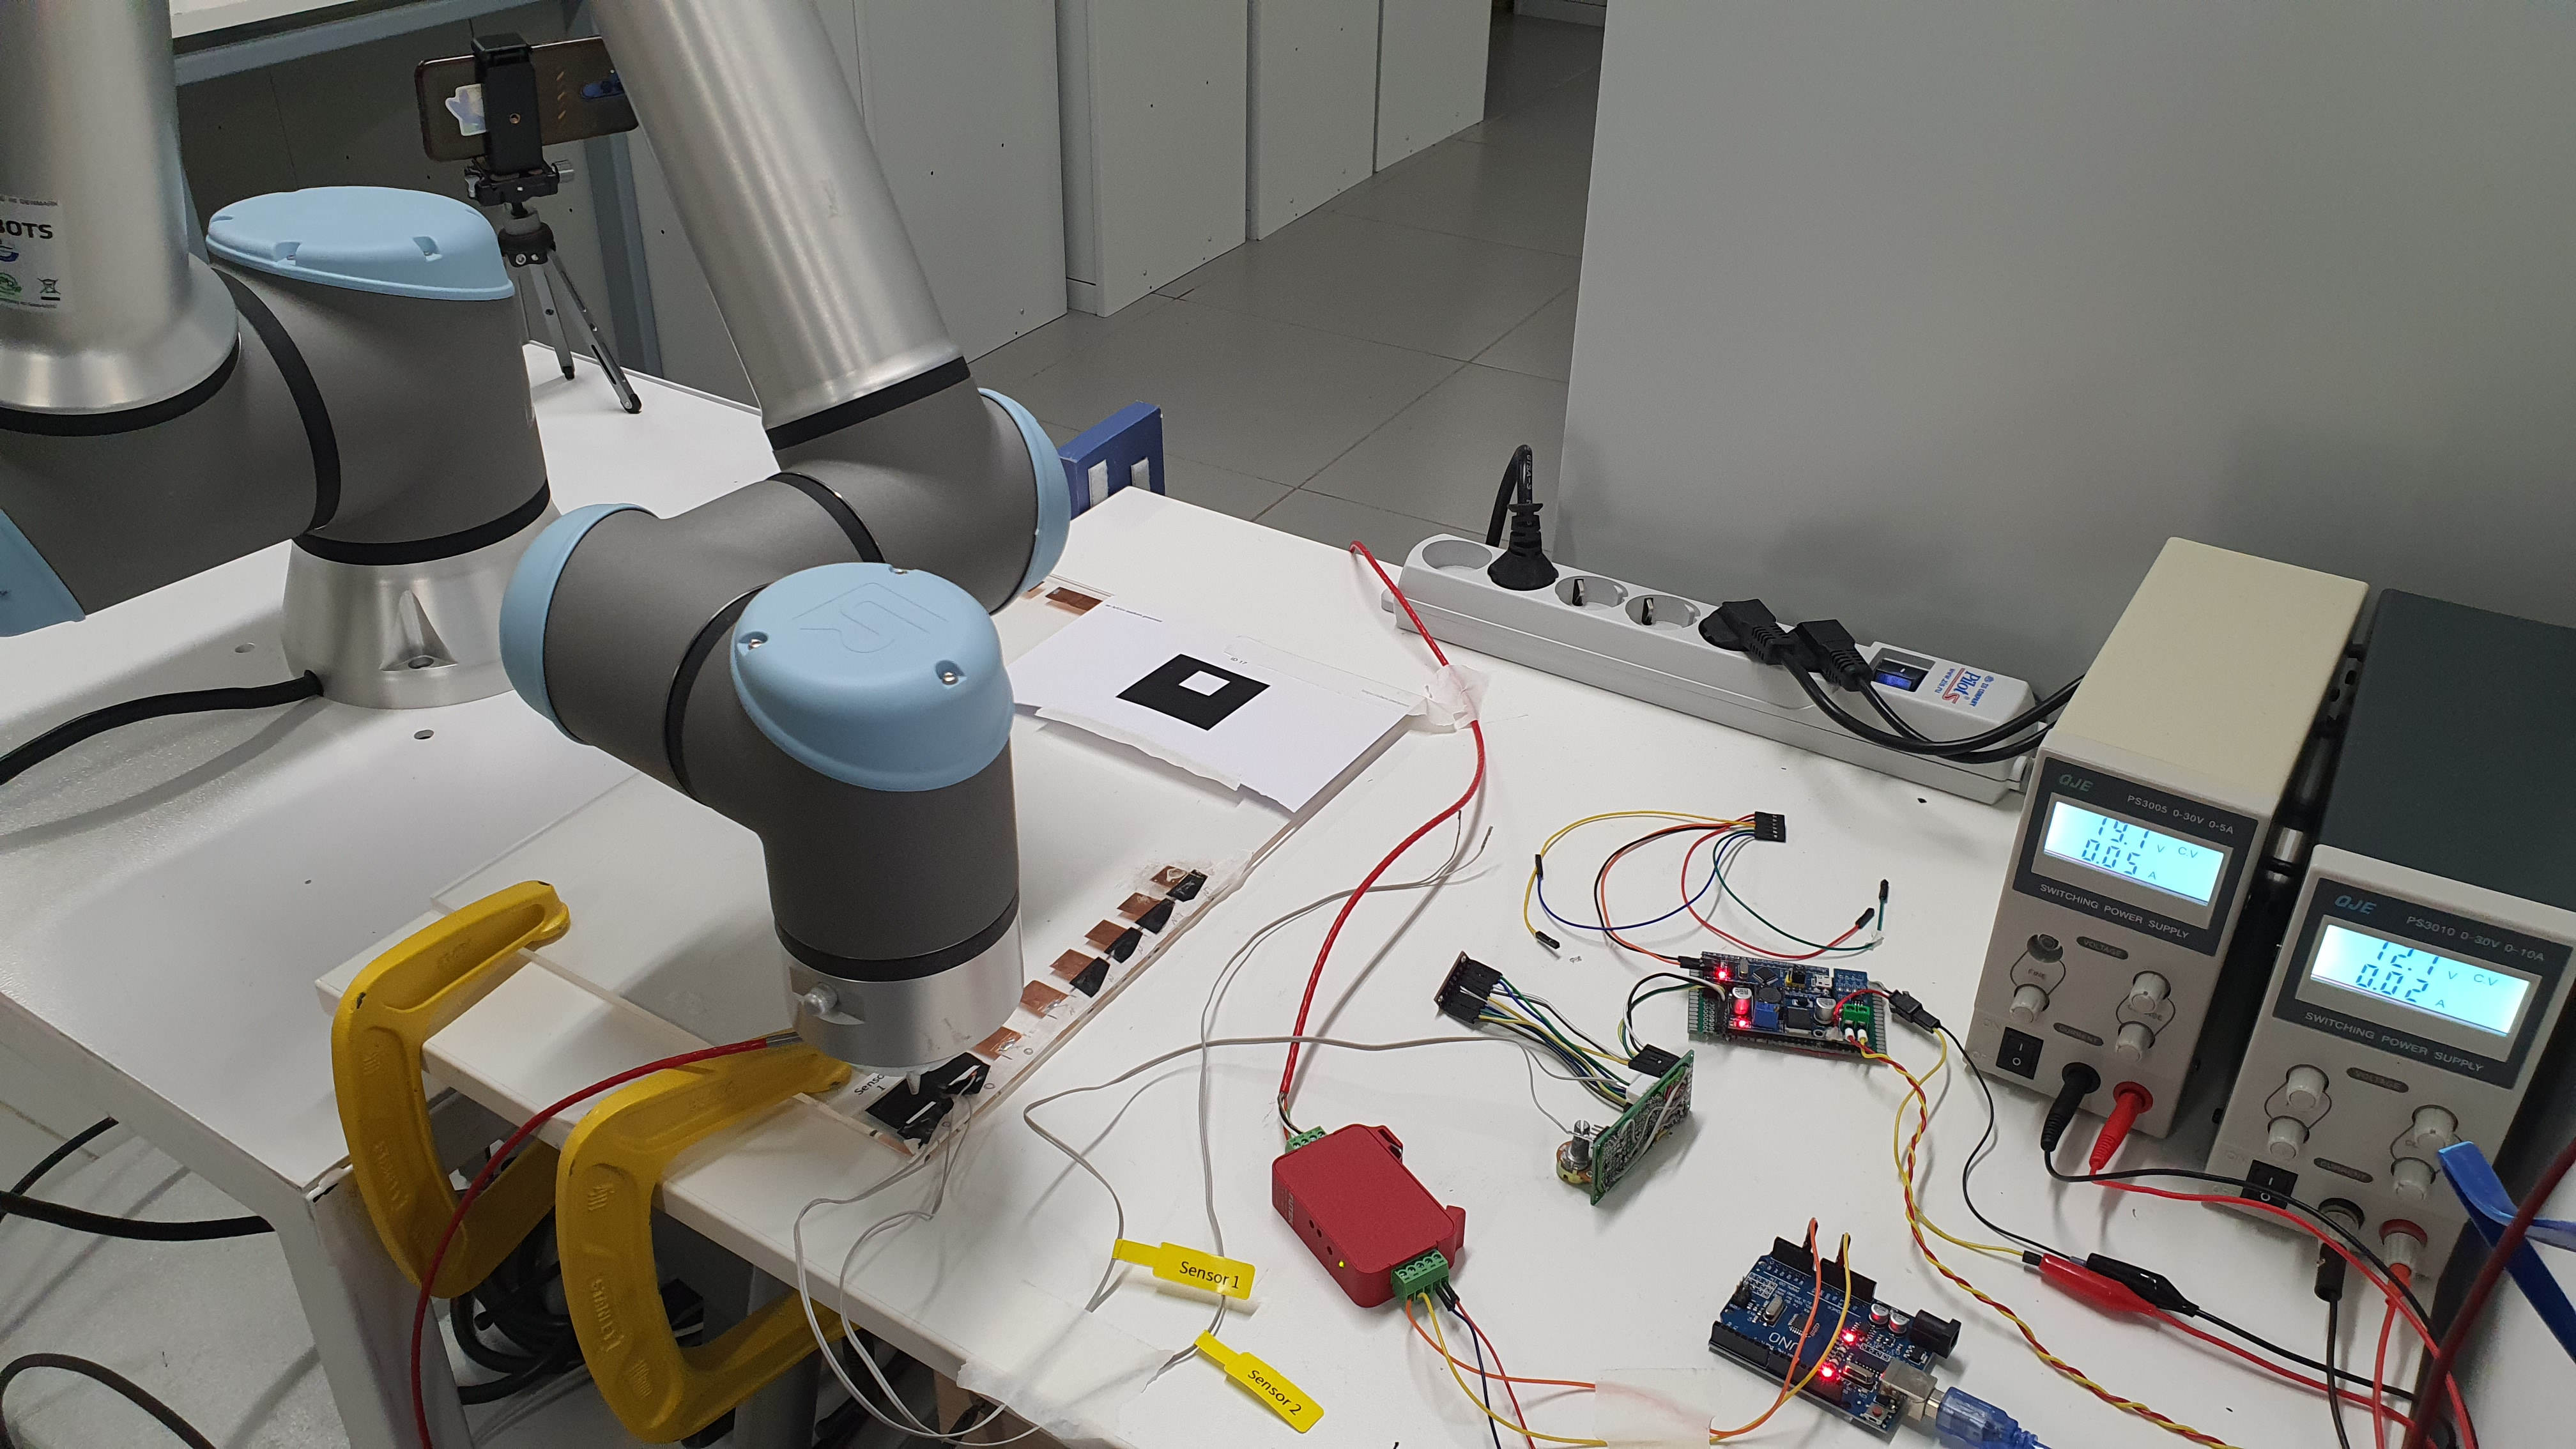
\includegraphics[height=10cm,width=1\textwidth,keepaspectratio]{exp_stand1}};

                % Create scope with normalized axes
                \begin{scope}[
                        x={($0.1*(image.south east)$)},
                        y={($0.1*(image.north west)$)}]
                    \draw[latex-, very thick,green] (3.5,2.2) -- (2.5,1)
                    node[rounded corners=3pt,below left,black,fill=white]{\small Velostat сенсор};

                    \draw[stealth-, very thick,green] (3.5,2.6) -- ++(-0.7,+0.5)
                    node[rounded corners=3pt,left,black,fill=white]{\small Датчик силы};

                    \draw[stealth-, very thick,green] (6.5,3) -- (7,6)
                    node[rounded corners=3pt,above right,black,fill=white]{\small Self-made PCB};

                    \draw[stealth-, very thick,green] (7.2,1.5) -- (8,5)
                    node[rounded corners=3pt,above right,black,fill=white]{\small Ардуино};

                    \draw[stealth-, very thick,green] (2.5,9.5) -- (4,9.5)
                    node[rounded corners=3pt,right,black,fill=white]{\small Камера};

                    \draw[very thick,green] (0.5,2.5) rectangle (4.2,9)
                    node[below left,black,fill=green]{\small UR10e};

                    \draw[latex-, very thick,green] (4.5,7.2) edge (5.5,7.5)
                    (4.8,5.3) -- (5.5,7.5)
                    node[rounded corners=3pt,above,black,fill=white]{\small Aruco маркеры};
                \end{scope}
            \end{tikzpicture}
            \caption{Общий вид экспериментального стенда}
            \label{fig:exp_standd}
        \end{subfigure}

        \begin{subfigure}{0.9\textwidth}
            \centering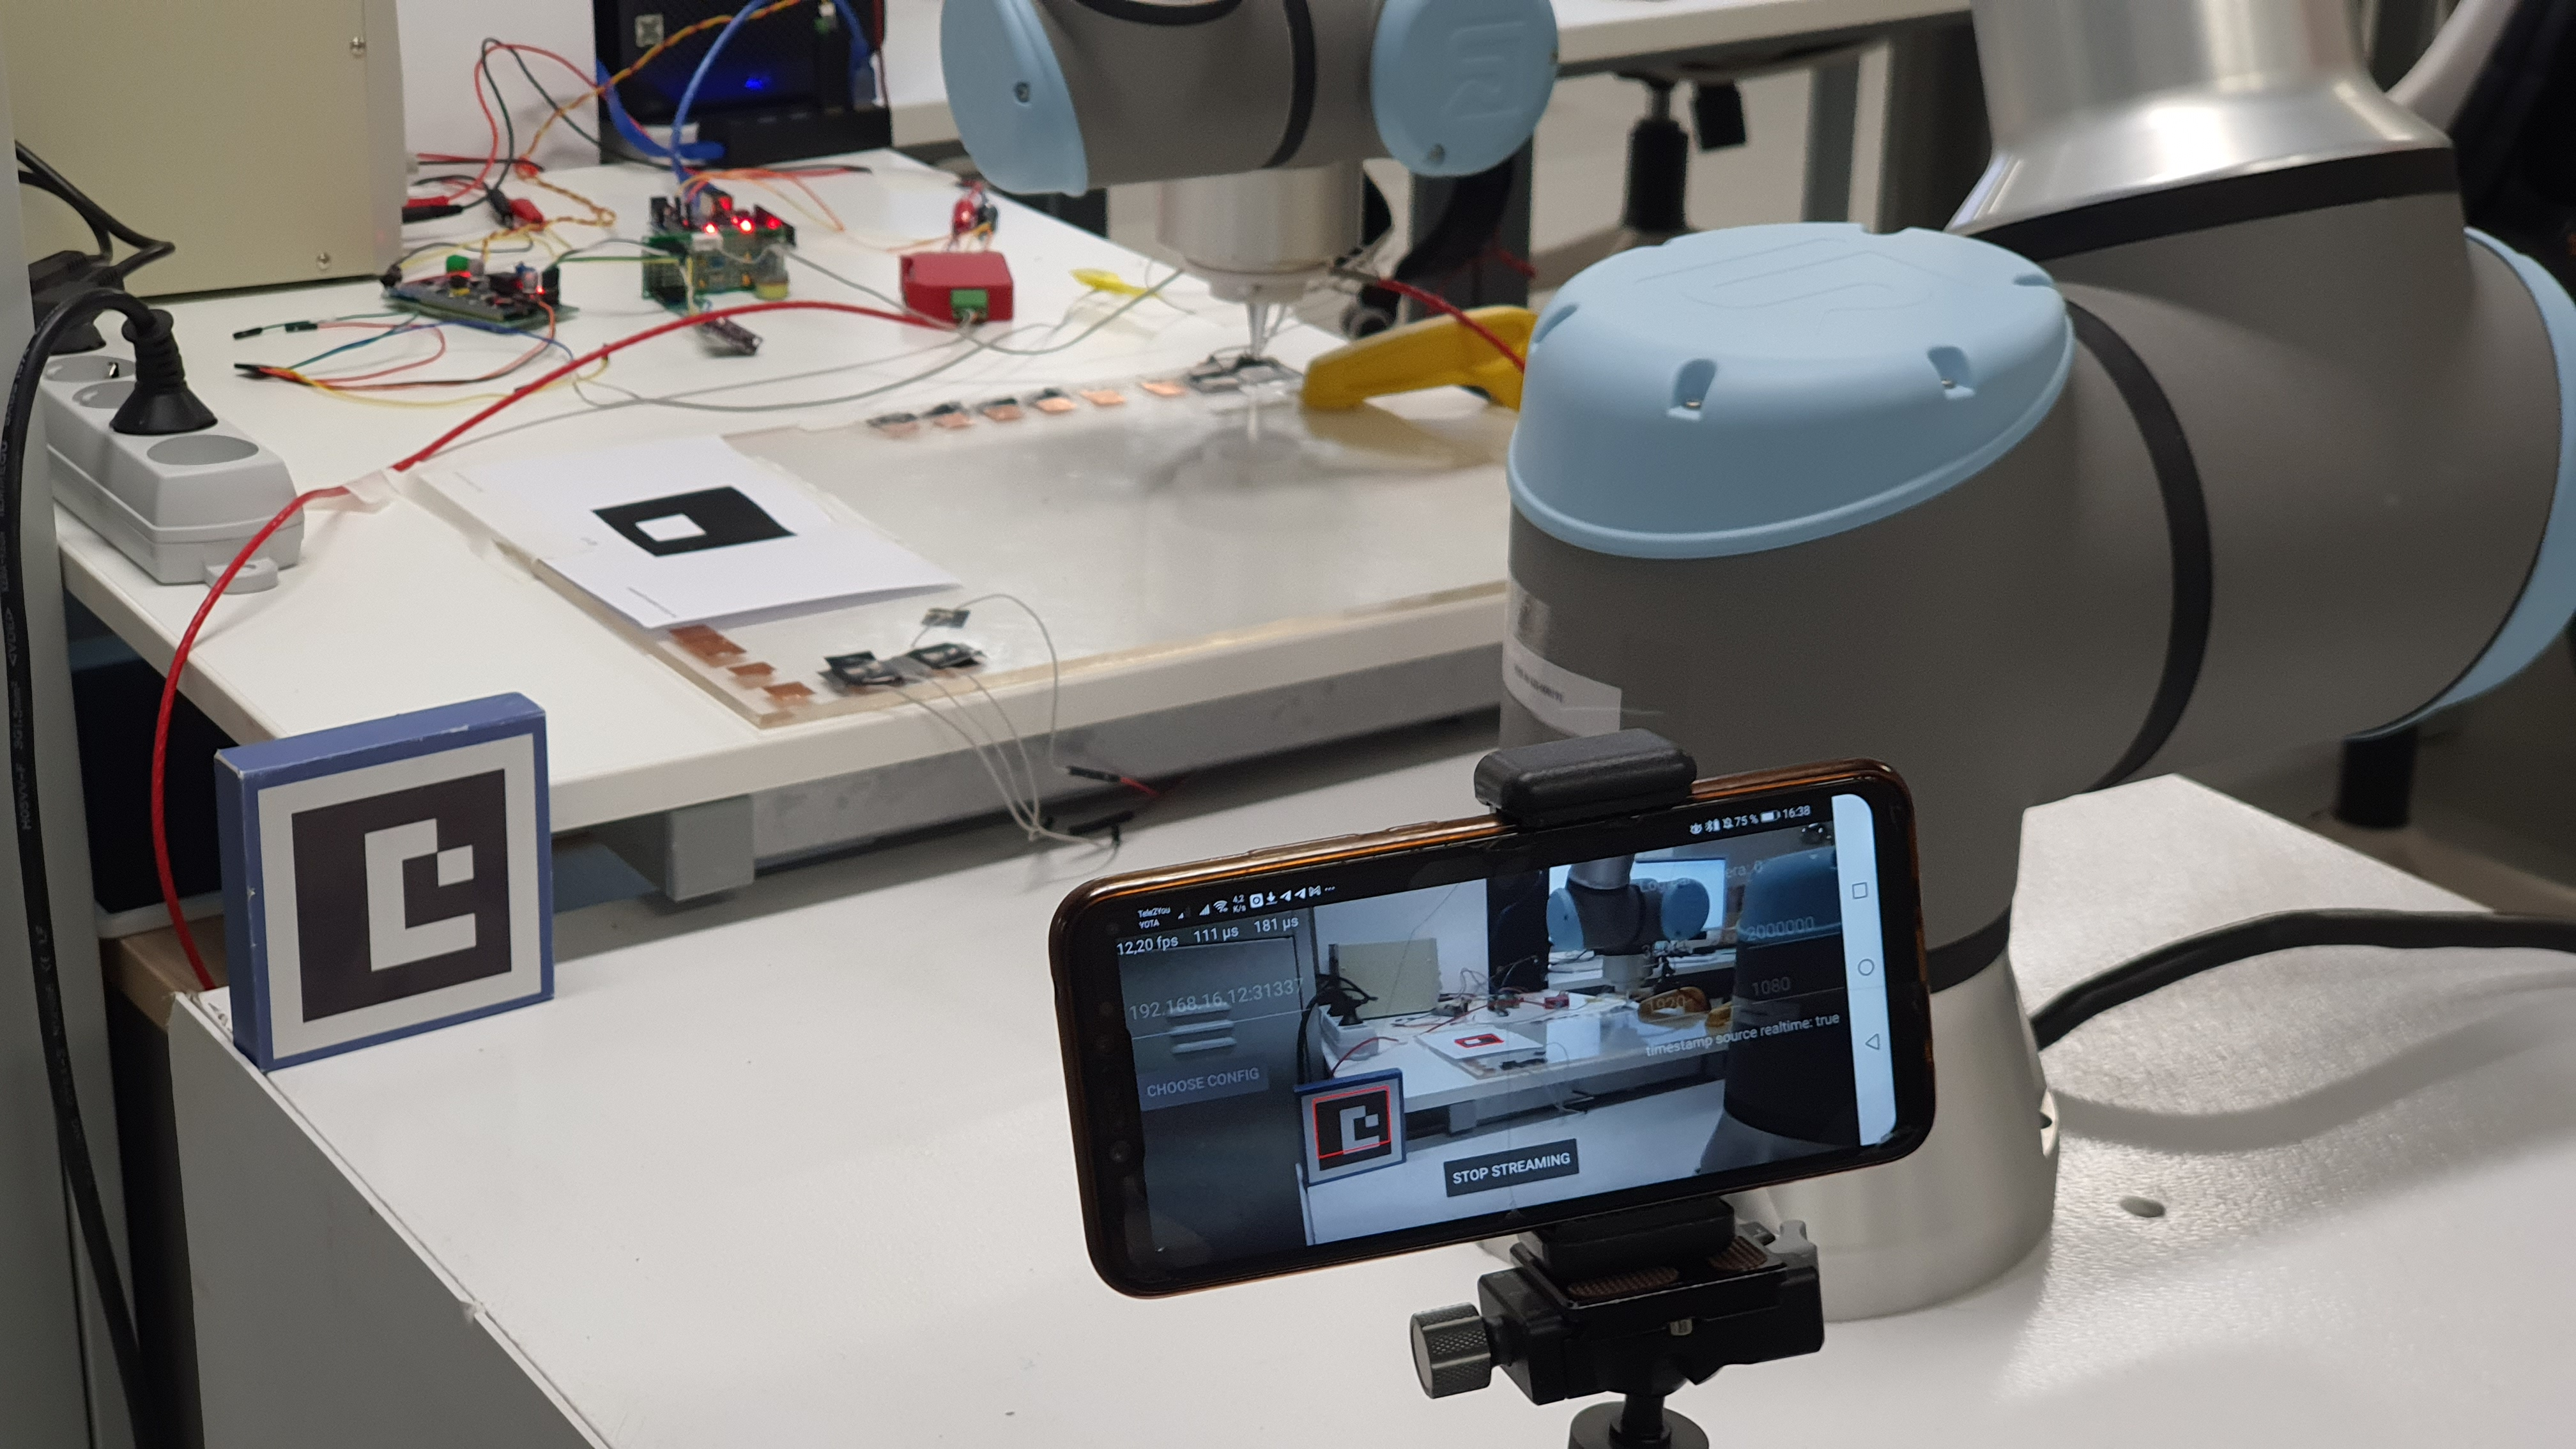
\includegraphics[height=10cm,width=1\textwidth,keepaspectratio]{exp_stand2}
            \caption{Способ нивелировать ошибку по углу с помощью Aruco маркеров}
            \label{fig:exp_stand2}
        \end{subfigure}
        \caption{Разработанный экспериментальный стенд}
\end{figure}

Для касания только части объекта исследования были разработаны различные насадки. Представленные размеры \pic{fig:all_end_effectors.png} были выбраны из-за размеров преобразователя. Ожидается, что минимальный размер пятна контакта движителя с жёсткой опорной поверхностью будет определяться податливостью материала самого движителя и составит порядка 2 мм. При контакте с более податливым грунтом площадь пятна контакта может быть намного больше, поэтому максимальный размер насадки ограничен размерами самого датчика.

\begin{figure}[H]
    \begin{subfigure}[t]{0.99\textwidth}
        \centering
        \begin{tikzpicture}
            % Include the image in a node
            \node [above right, inner sep=0] (image) at (0,0)
            {\centering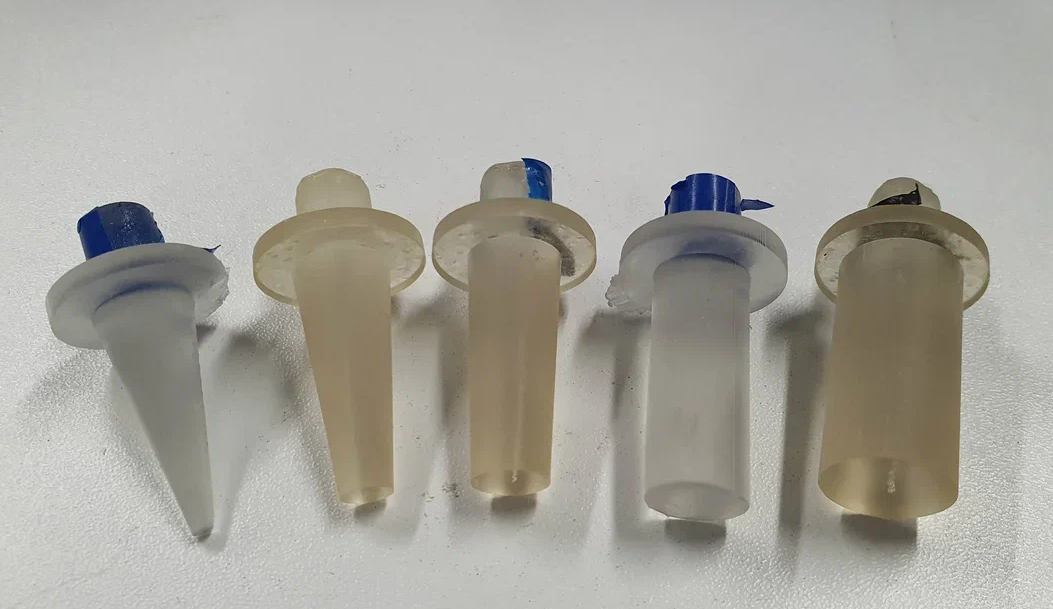
\includegraphics[height=10cm,width=1\textwidth,keepaspectratio]{all_end_effectors.png}};
            % Create scope with normalized axes
            \begin{scope}[
                    x={($ 0.1*(image.south east)$)},
                    y={($ 0.1*(image.north west)$)}]
                \node[rounded corners=3pt,black,fill=white] at (1.1,7.4){\tiny 2 mm };
                \node[rounded corners=3pt,black,fill=white] at (3.1,7.9){\tiny 6 mm };
                \node[rounded corners=3pt,black,fill=white] at (4.9,8.1){\tiny 8 mm };
                \node[rounded corners=3pt,black,fill=white] at (6.7,7.9){\tiny 12 mm };
                \node[rounded corners=3pt,black,fill=white] at (8.6,7.9){\tiny 15 mm };
            \end{scope}
        \end{tikzpicture}
        \caption{Насадка для нажатия объект
            исследования с диаметром нажатия меньше, чем сам объект}
        \label{fig:all_end_effectors.png}
    \end{subfigure}

    \begin{subfigure}[t]{0.99\textwidth}
        \centering
        \begin{tikzpicture}

            % Include the image in a node
            \node [
                above right,
                inner sep=0] (image) at (0,0) {\centering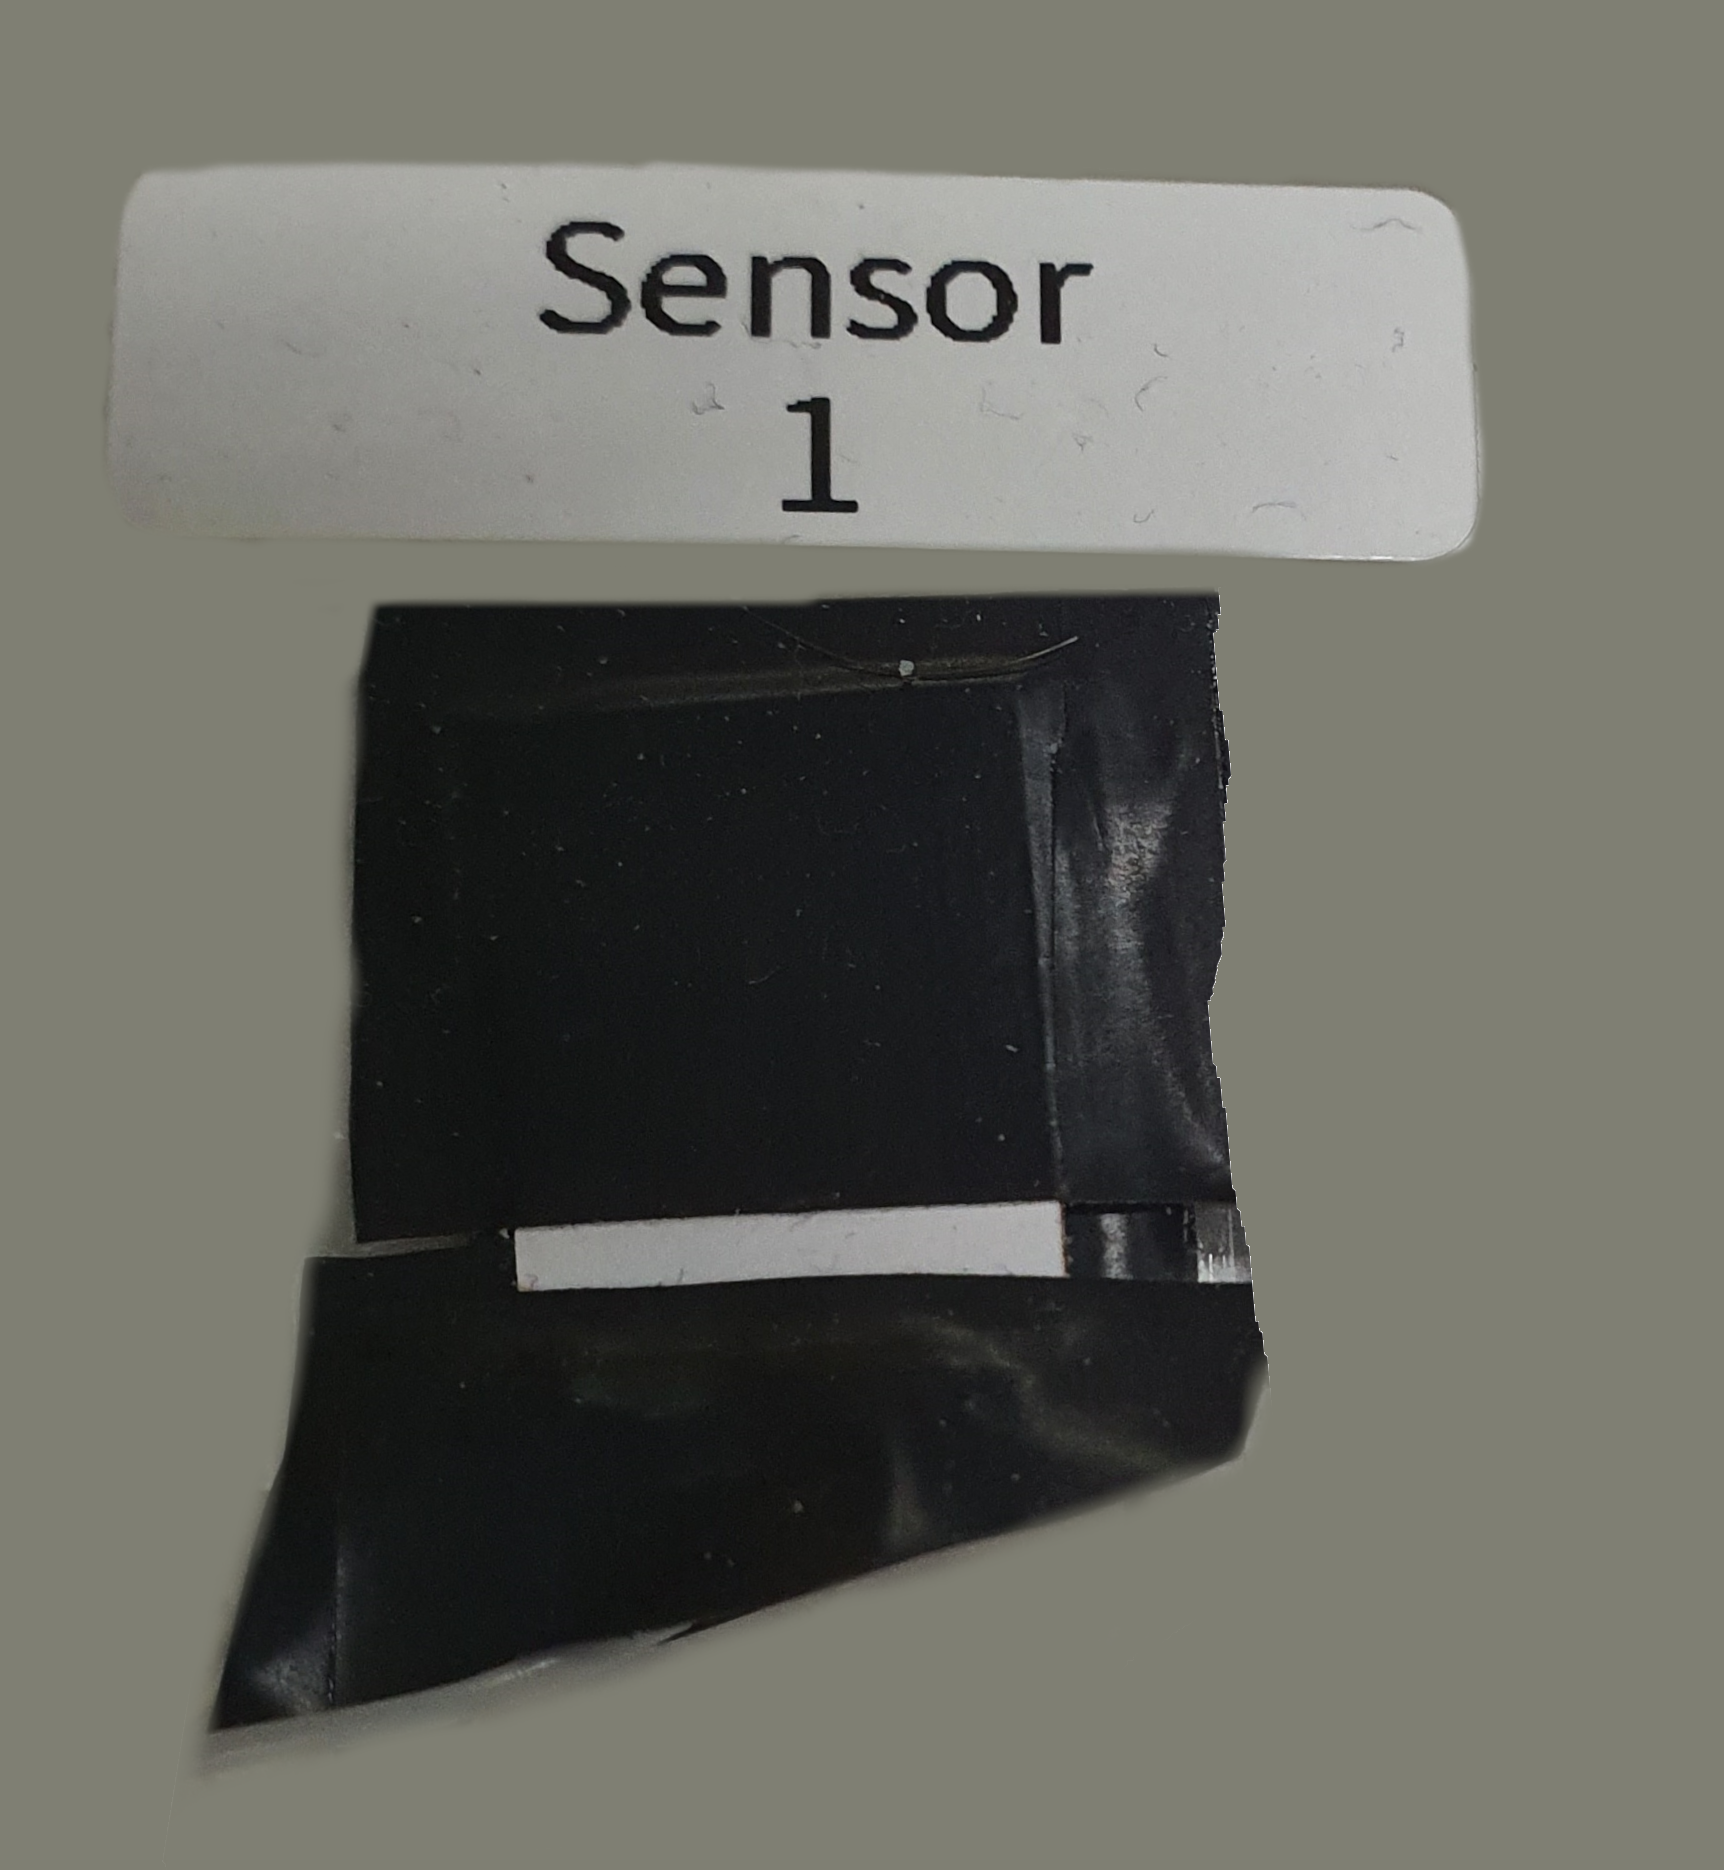
\includegraphics[height=8cm,width=1\textwidth,keepaspectratio]{sensors_grid.png}};

            % Create scope with normalized axes
            \begin{scope}[
                    x={($0.1*(image.south east)$)},
                    y={($0.1*(image.north west)$)}]
                \draw [green, very thick,
                    decorate,
                    decoration = {brace,
                            raise=5pt,
                            amplitude=5pt,
                            aspect=0.5}] (6,3.7) --  (3,3.7)
                node[pos=0.5,below=10pt,green]{$15\ mm$};

                \draw [green, very thick,
                    decorate,
                    decoration = {brace, mirror,
                            raise=5pt,
                            amplitude=5pt,
                            aspect=0.5}] (6,3.6) --  (6,6.4)
                node[pos=0.5,right=10pt,green]{$15\ mm$};

                \draw[green,step=1,xshift=34, yshift=43]  (0.5,0.5) grid +(3,3);

                \node[circle,fill=green,scale=0.4] at (3.3,6.27){\small 1};
                \node[circle,fill=green,scale=0.4] at (5.92,3.7){\small 16};
            \end{scope}

        \end{tikzpicture}
        \caption{Сенсор представлен \\ как $4\times4$ сетка}
        \label{fig:sensor_grid}
    \end{subfigure}
    \caption{Представление места нажатия инструментом сенсора и сам инструмент}
\end{figure}

Импедансное управление состоит из двух блоков -- модификация траектории для оси $z$, начиная с\eqref{eq:traj_mod}, и управление по скорости -- с \eqref{eq:vel_control}.

\begin{align}
    \label{eq:traj_mod}
    X_s^0 = 0, \dot{X}_s^0 =0,  X_g^k, \dot{X}_g^k \text{ -- goal state}, X_s = X_g - X_d \\
    X_g = X_g^0 + \frac{F_d}{\eta } \\
    \dot{X}_s + \eta  X_s = F^k \\
    X_s^k = odeint(X_s^{k-1},t,F^k), t = [0,dT] \\
    X_s^{k-1} = X_s^k;  \dot{X}_s = f(X_s,t,F^k) \\
    X_d = X_g - X_s; \dot{X}_d = \dot{X}_g - \dot{X}_s
\end{align}

\begin{align}
    \label{eq:vel_control}
    X_d = \begin{bmatrix}
        x_g \\ y_g \\ z_d
    \end{bmatrix} \\
    U = \dot{X}_d + K(X_d - X), \\ \text{ where } X=get\_state(); \\ 
    set\_speed(U)
\end{align}

На рисунке ниже \pic{fig:force_data_pos.png} представлен результат работы импедансного управления на частоте 450 $Hz$. Необходимая сила нажатия --- $17\ H$.
\begin{figure}[H]
        \centering
         \begin{tikzpicture}
            % Include the image in a node
            \node [above right, inner sep=0] (image) at (0,0) 
            {\centering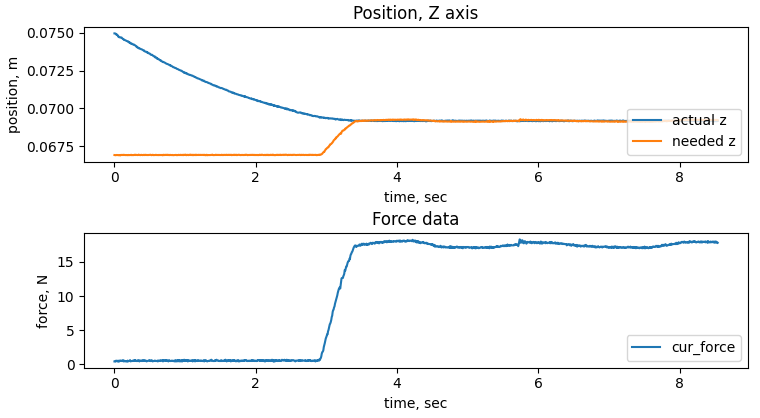
\includegraphics[height=10cm,width=1\textwidth,keepaspectratio]{force_data_pos.png}};          
            % Create scope with normalized axes
            \begin{scope}[
                x={($ 0.1*(image.south east)$)},
                y={($ 0.1*(image.north west)$)}]
                \draw[thick,green, dashed] (4.2,1) -- (4.2,8)
                node[above right,black,fill=white]{\tiny Касание с поверхностью};
            \end{scope}
        \end{tikzpicture}
        \caption{Графики зависимости силы и позиции по $z$ от времени во время эксперимента по исследованию Velostat}
        \label{fig:force_data_pos.png}
    \end{figure}

\section{Экспериментальная часть}

В исследовании были проведены.
\begin{enumerate}
    \item \textbf{Статический эксперимент}. Цель — определить коэффициенты для математической модели преобразователя. Для этого на сенсор кладется известная нагрузка на 60 секунд (за это время можно явно наблюдать гистерезис) и собираются данные с преобразователя;
          \item\textbf{Динамический эксперимент}. Цель — определить влияние показаний сенсора в зависимости от положения площадки контакта. Для этого преобразователь представлен в виде матрицы $4 \times 4$. Размер преобразователя в эксперименте 15 на 15 мм. Манипулятор нажимает на преобразователь с одинаковым давлением на протяжении всех экспериментов в различные позиции на преобразователе, используя пять различных насадок (диаметр окружности от 2 мм до 15 мм) \pic{fig:sensor_grid}.
\end{enumerate}


Статическим экспериментом проверялась формула \eqref{eq:velostat_eqn}. Из-за гистерезиса необходимо учитывать время нажатия на объект. При приложении на сенсор постоянной силы показания сенсора будут меняться.
\begin{align}
    \label{eq:velostat_eqn}
    V_{out} = V_0 + p[k_p + k_e(1-e^\frac{-(t-t_0)}{\tau_{res}})](1-e^{-\frac{A}{p}}) \\
    k_p = A_1e^{-A_2p}; \tau_{res} = B_0 + B_1e^{-\frac{p}{B_2}}
\end{align}
где,  \nom{$V_0$}{начальное напряжение}, \nom{$p,\ A_i,\ B_i,\ \tau_{res},\ k_i$}{настраиваемые константы}, \nom{$t$}{текущее время}, \nom{$t_0$}{время начала нажатия}.
Для решения задачи регрессии использовался устойчивый нелинейный метод наименьших квадратов. Результат представлен ниже \pic{fig:least_square_model.png}.

\begin{figure}[H]
    \centering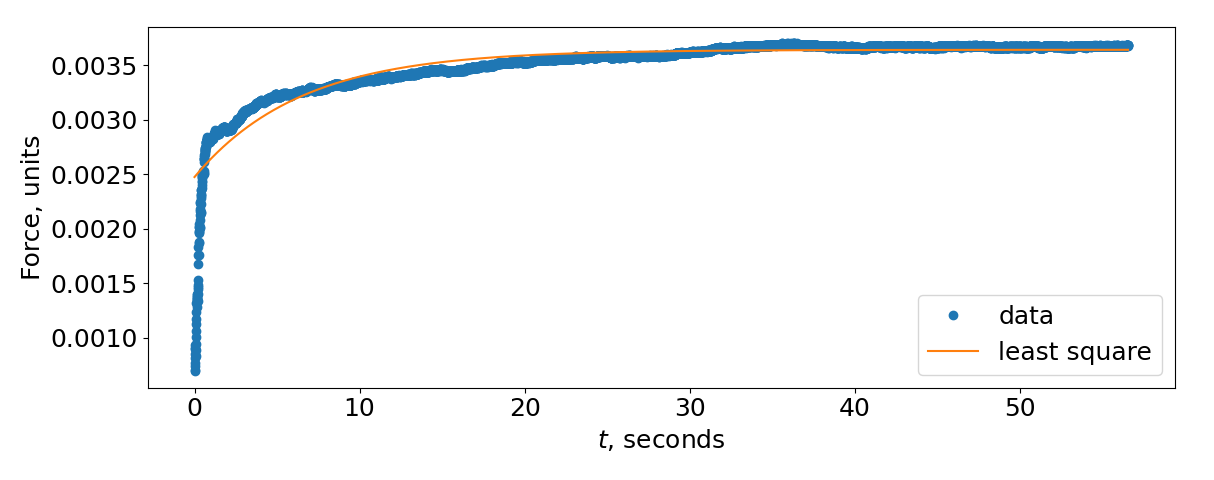
\includegraphics[height=10cm,width=1\textwidth,keepaspectratio]{least_square_model.png}
    \caption{Результаты статического эксперимента}
    \label{fig:least_square_model.png}
\end{figure}

Ниже \pic{fig:dynamics_exp} представлены некоторые результаты распределения ошибок по площади сенсора при взаимодействии с насадками разных размеров. Ошибки определялись как нормализованная разница между показаниями калиброванного сенсора силы Futek и исследуемого преобразователя на базе Velostat. На рисунке \ref{fig:sens1_pike1} показаны ошибки для насадки диаметром 2 мм, а на рисунке \ref{fig:sens1_pike3} — для насадки диаметром 8 мм.

\begin{figure}[H]
    \centering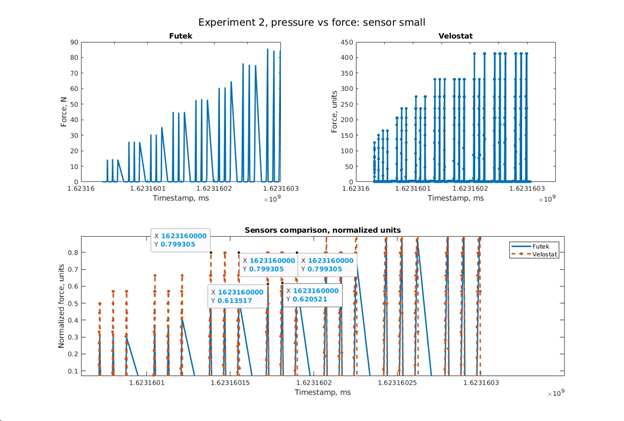
\includegraphics[width=0.99\textwidth]{sensor_sensor.png}\\
    \caption{Проверка чувствительности датчика. Слева - идеальные данные, справа - результат, полученный с помощью созданного датчика.}
    \label{fig:sensor_sensor}
    \end{figure}

Можно заметить, что в \ref{fig:sens1_pike3} максимальная разница нормированных показаний между Futek и Velostat --- 19\% единиц. В остальных ячейках разница значений не превышает 10\%. Такая же тенденция продолжается как и при увеличении размера насадки, так и на других сенсорах.


\begin{figure}[H]
    \begin{subfigure}{0.99\textwidth}
        \centering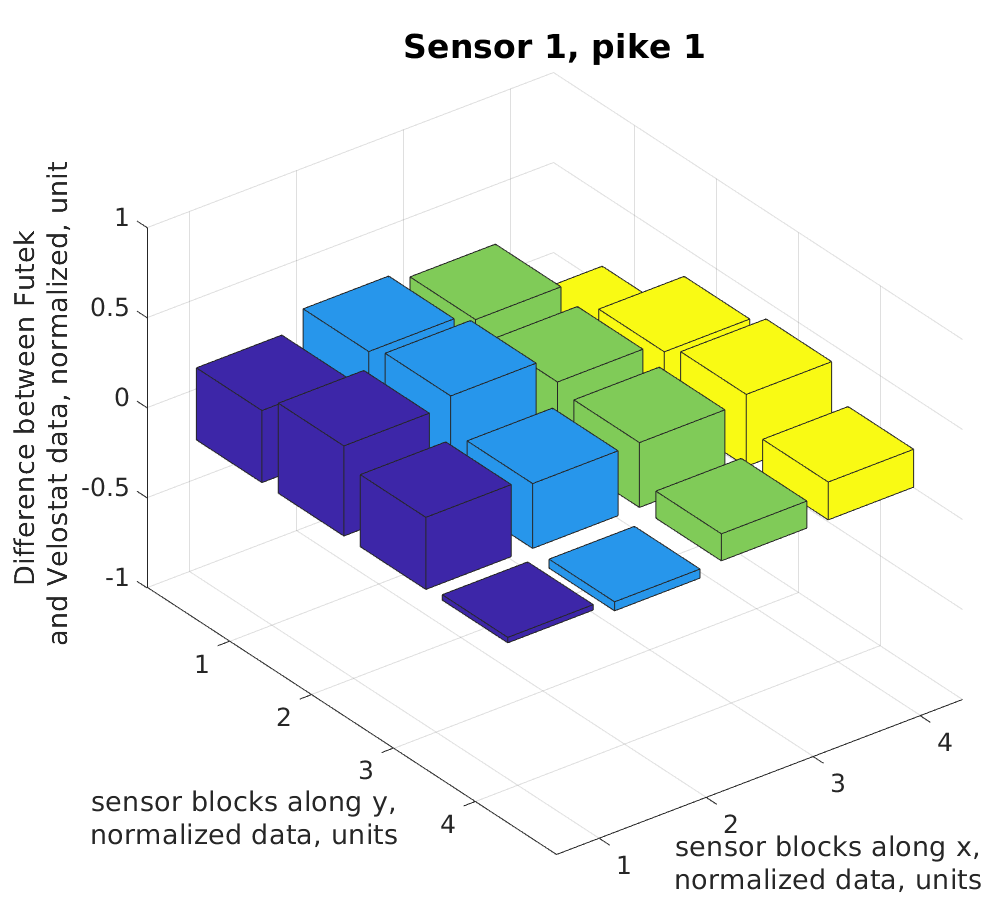
\includegraphics[height=10cm,width=1\textwidth,keepaspectratio]{sens1_pike1.png}
        \caption{диаметр насадки равный 2 мм }
        \label{fig:sens1_pike1}
    \end{subfigure}

    \begin{subfigure}{0.99\textwidth}
        \centering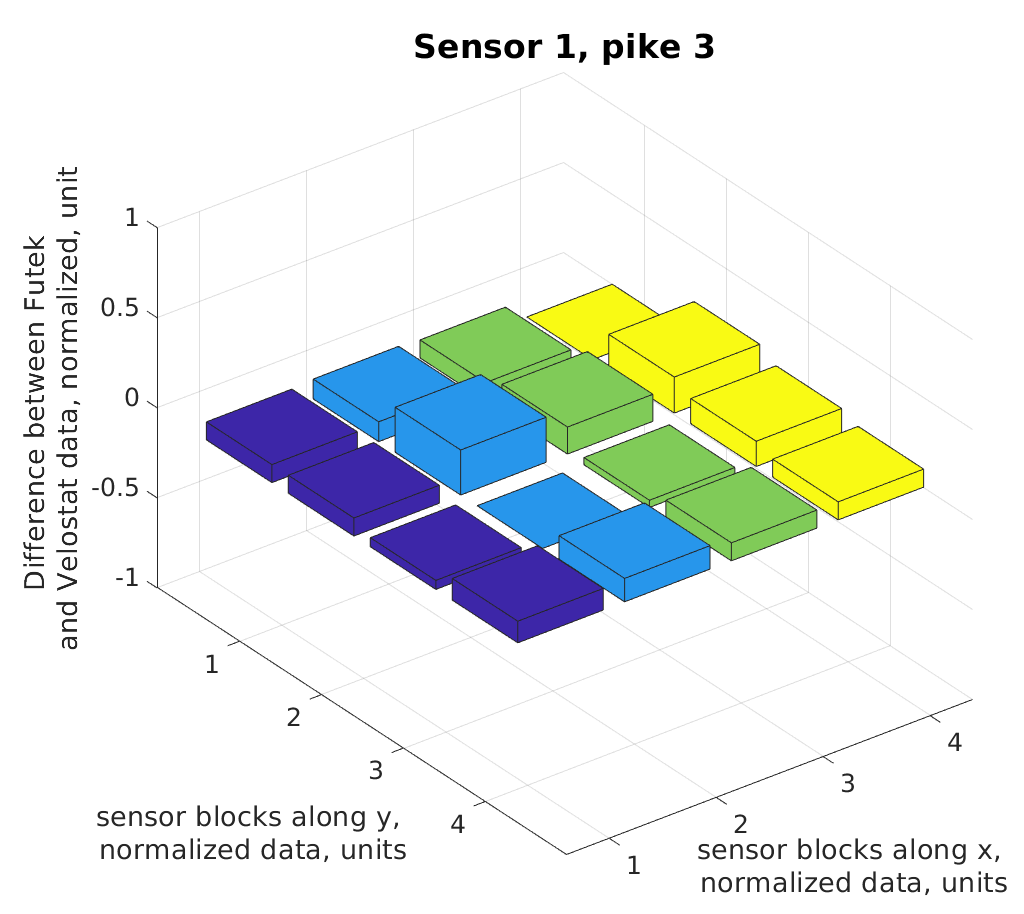
\includegraphics[height=10cm,width=1\textwidth,keepaspectratio]{sens1_pike3.png}
        \caption{Диаметр насадки равный 8 мм }
        \label{fig:sens1_pike3}
    \end{subfigure}
    \caption{Динамический эксперимент}
    \label{fig:dynamics_exp}
\end{figure}

Результатом данной главы является описание разработки пьезорезистивного датчика на основе Velostat. Описана и обоснованна экспериментальная установка для определения силы нажатия на часть сенсора. Для экспериментальной установки была разработана система управления,а также методика работы. 

Были успешно проведены два эксперимента, целью первого являлось определение коэффициентов для математической модели преобразователя. А для второго --- определить влияние показаний сенсора в зависимости от положения площадки контакта. 

По результатам исследований показано, что характеристики преобразователя удовлетворяют требованиям к системе тактильного восприятия шагающего робота  по точности и отзывчивости, когда ожидаемый размер площади контакта превышает 25 процентов площади преобразователя.